\documentclass{report}
\date{Mars 2024}
\author{Léo MANTION, Eymeric VINET, Quentin TOMAS}
\title{Projet de Jeu Vidéo en 2D : JumpCraft}
\usepackage[french]{babel}
\usepackage[T1]{fontenc}
\usepackage[a4paper,top=2cm,bottom=2cm,left=3cm,right=3cm,marginparwidth=1.75cm]{geometry}
\usepackage{amsmath}
\usepackage{graphicx}
\usepackage{enumitem}
\usepackage[colorlinks=true, allcolors=blue]{hyperref}
\renewcommand{\thesection}{\arabic{section}}

\makeatletter
\renewcommand{\maketitle}{
  \begin{titlepage}
    \begin{flushleft}
      \includegraphics[width=8cm]{universite-de-montpellier.jpg}
    \end{flushleft}
    \vspace{4cm}
    \centering
    {\huge \bfseries \@title \par}
    \vspace{1cm}
    {\Large \@author \par}
    \vspace{1cm}
    {\large \@date \par}
    \vfill\null
  \end{titlepage}
}
\makeatother

\begin{document}

\maketitle

\tableofcontents
\begin{figure}
    \centering
    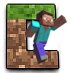
\includegraphics[width=0.25\linewidth]{Logo.png}
    \centering
    
\includegraphics[width=0.5\linewidth]{Godot.png}
\end{figure}
\clearpage

\section{Introduction}

Notre groupe a pour projet de créer un jeu vidéo de type plateforme en 2D vue de côté, s’inspirant du jeu Minecraft pour le thème graphique de celui-ci. Le principe du jeu se rapprochera du jeu indépendant Jump King dont le but est d’atteindre le sommet du niveau en sautant de plateforme en plateforme sans tomber. Pour ce faire, nous allons utiliser le moteur de jeu multiplateforme Godot qui nous permettra de créer le contenu du jeu.

L’objectif de ce projet est donc de créer un jeu simple, accessible à tout le monde, mais possédant quand même une certaine difficulté et une notion d’apprentissage du niveau. En effet, la chute du joueur dans le niveau l’emmènera plus bas dans celui-ci, l’obligeant alors à refaire certaines parties.

Nous avons décidé de partir dans la création d’un jeu vidéo par rapport à nos ambitions personnelles et nos futurs projets professionnels. Comme nous avions également bien aimé le principe du jeu vidéo Jump King, nous avons décidé de lui rendre hommage en créant notre propre version du jeu.

\vspace{1cm}

\section{Description Générale du Projet}

\vspace{0.5cm}

\subsection{Pour ce projet, nous aurons à développer :}

\begin{itemize}[label={\textbf{--}}]
    \item les mouvements du personnage jouable, à savoir les directions qu’il peut emprunter (gauche, droite, saut).
    \item Des hitbox sur les différents obstacles présents dans le jeu ainsi que sur le joueur.
    \item Un niveau avec les différentes plateformes et chemins disponibles, avec une difficulté progressive pour donner un sentiment d’accomplissement et de progression au joueur.
    \item Un système de saut intéressant pour se déplacer entre les plateformes et progresser dans le niveau.
\end{itemize}

\vspace{1cm}

\section{Spécifications fonctionnelles}

\vspace{0.5cm}

\subsection{Pour les mécaniques de jeu :}

\begin{itemize}[label={\textbf{--}}]
    \item Le joueur contrôle un personnage qui peut sauter de plateforme en plateforme.
    \item Les sauts sont affectés par la durée d'appui sur les touches de déplacement.
\end{itemize}

\subsection{En ce qui concerne le niveau :}

\begin{itemize}[label={\textbf{--}}]
    \item Il n’y aura qu’un seul niveau sur toute la durée du jeu, mais il aura une certaine longueur.
    \item Le joueur pourra progresser dans le niveau uniquement par voie verticale et non horizontale.
    \item Le niveau sera conçu pour augmenter progressivement en difficulté.
\end{itemize}

\subsection{Pour l’interface utilisateur :}

\begin{itemize}[label={\textbf{--}}]
    \item Il y aura un menu principal dans lequel le joueur pourra reprendre sa partie ou quitter le jeu.
    \item Le temps de jeu sera affiché dans un coin de l’écran du joueur pour lui indiquer combien de temps, il a passé pour compléter le niveau.
    \item L’interface pendant les temps de jeu sera minimaliste afin de ne pas déranger le joueur.
    \item Un menu pause sera disponible pour le joueur afin que celui-ci puisse sauvegarder, reprendre le jeu ou retourner au menu principal.
\end{itemize}

\begin{figure}
    \centering
    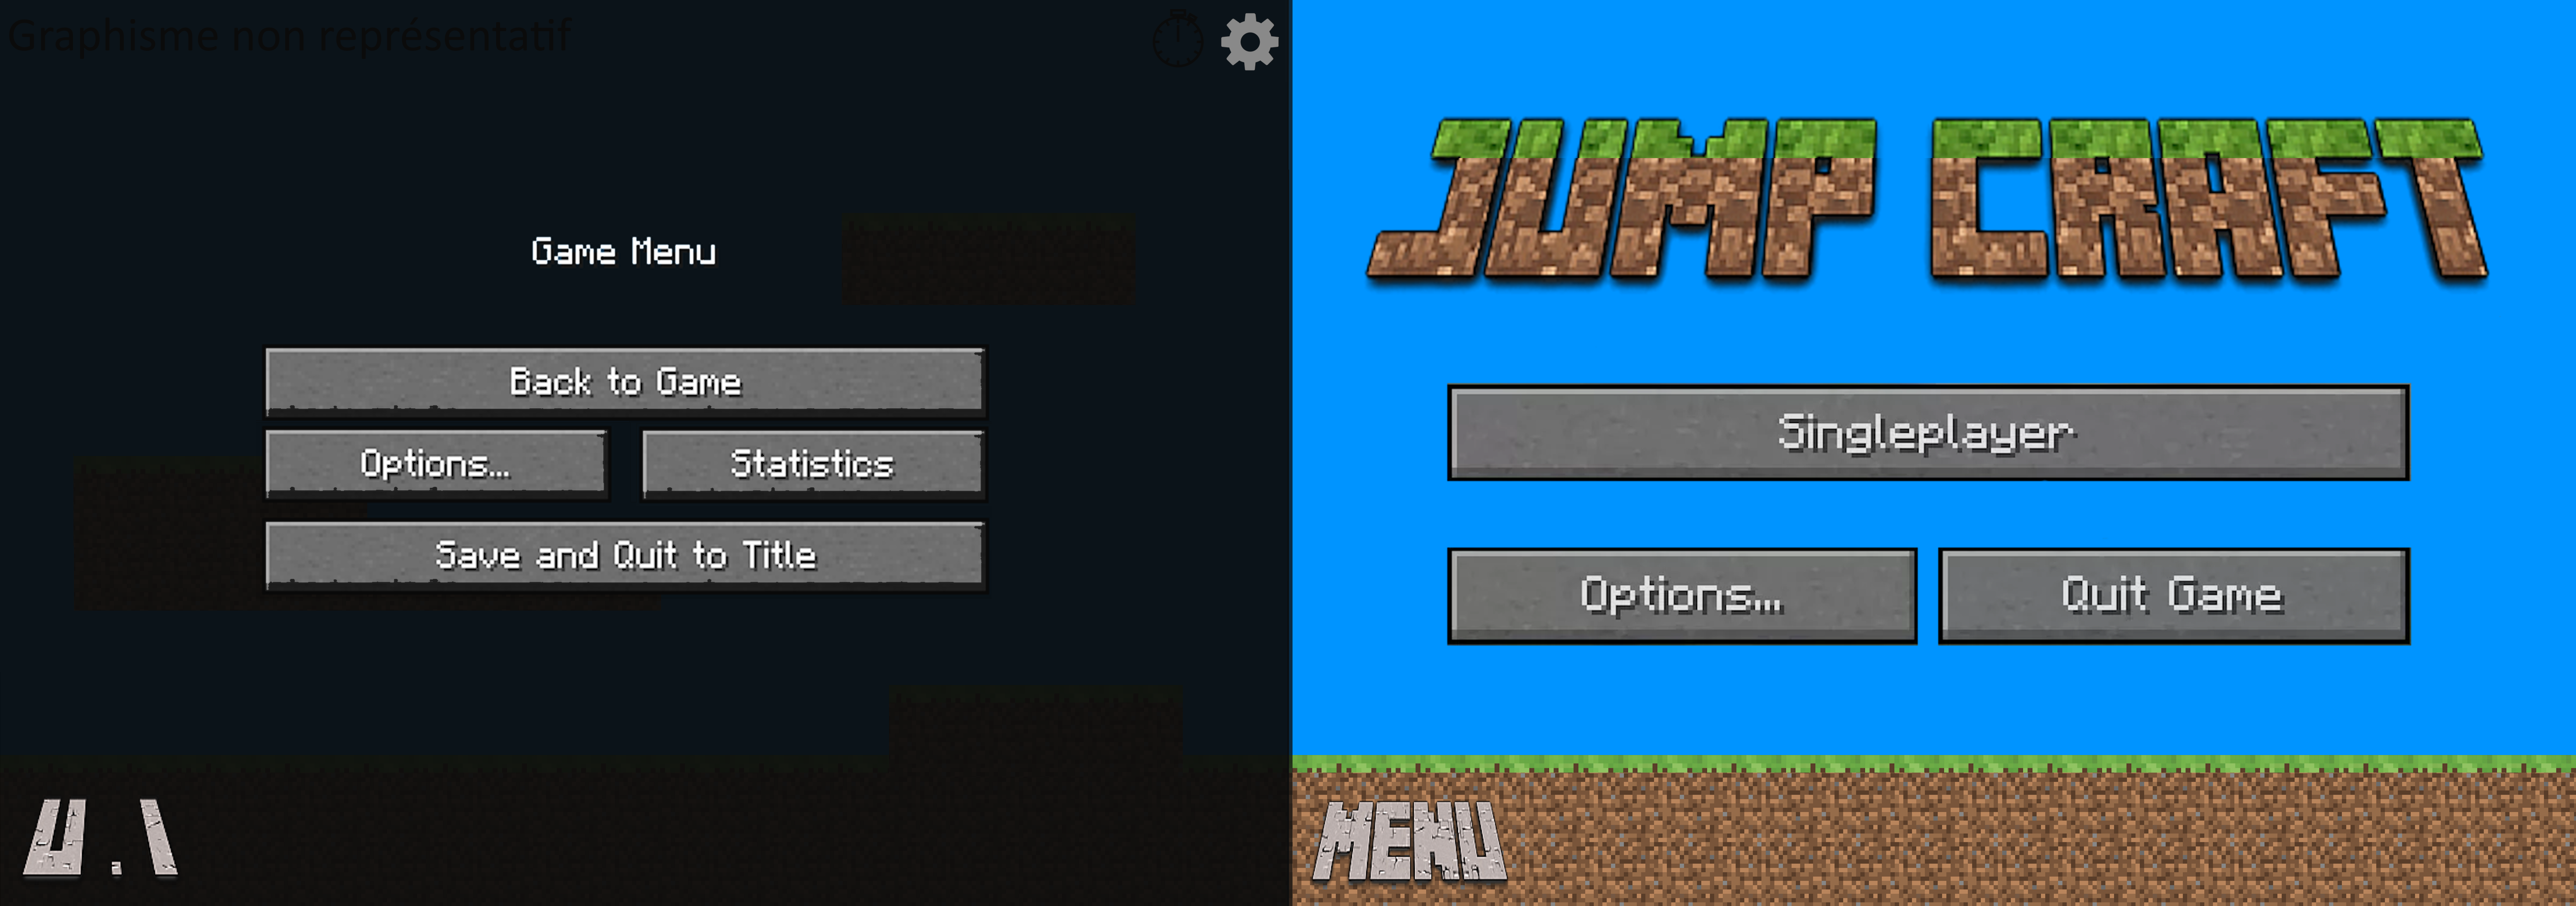
\includegraphics[width=1\linewidth]{UI_&_Menu.png}
    
\end{figure}

\vspace{1cm}

\section{Spécifications techniques}

\vspace{0.5cm}

\subsection{Moteur de jeu :}

\begin{itemize}[label={\textbf{--}}]
    \item Nous utiliserons le moteur de jeu multiplateforme Godot qui contient déjà un moteur 2D, un moteur physique et un gestionnaire d’animation qui nous aideront pendant le développement. 
\end{itemize}

\subsection{Langage de programmation utilisé :}

\begin{itemize}[label={\textbf{--}}]
    \item Nous utiliserons le langage de script GDScript pour la programmation du jeu dans Godot. 
    \item Nous devrons faire en sorte que les scripts soient organisés de manière à garantir une maintenance facile si jamais nous rencontrons des problèmes durant le développement. 
\end{itemize}

\subsection{Ressources graphiques :}

\begin{itemize}[label={\textbf{--}}]
    \item Nous utiliserons exclusivement des graphismes 2D pour les personnages, les décors et les animations.
    \item Nous utiliserons exclusivement des graphismes 2D pour les personnages, les décors et les animations.
\end{itemize}

\subsection{Contrôles :}

\begin{itemize}[label={\textbf{--}}]
    \item Le jeu se jouera exclusivement au clavier.
    \item Les contrôles seront entièrement configurables par le joueur.
\end{itemize}

\vspace{1cm} 

\section{Contraintes de développement}

\vspace{0.5cm}

\subsection{Méthodologie du développement}

\begin{itemize}[label={\textbf{--}}]
    \item Pour développer notre projet, nous fonctionnerons étape par étape et corrigerons les erreurs précédemment faites si jamais nous rencontrons des problèmes. Nous aurons donc une méthodologie qui se rapproche grandement de celle en cascade.
    \item Pour développer notre projet, nous fonctionnerons étape par étape et corrigerons les erreurs précédemment faites si jamais nous rencontrons des problèmes. Nous aurons donc une méthodologie qui se rapproche grandement de celle en cascade.
    \item \href{https://ibb.co/9bTFNWF}{Planning}
\end{itemize}

\vspace{1cm}

\section{Validation et tests}

\vspace{0.5cm}

\subsection{Stratégie de validation et test du système :}

\begin{itemize}[label={\textbf{--}}]
    \item Nous testerons à chaque nouvel ajout que le jeu ne présente aucun problème avant de passer à la suite de son développement.
\end{itemize}

\subsection{Critère d’acceptation du projet :}

\begin{itemize}[label={\textbf{--}}]
    \item Lorsque nous aurons atteint la dernière étape de notre projet et que celle-ci ne présentera pas de problème lors de son exécution (et celle de l’entièreté du programme) alors nous considèrerons le projet comme accompli et validé.
\end{itemize}

\vspace{1cm}

\section{Annexes}

\vspace{0.5cm}

\subsection{Document utilisé pour apprendre à utiliser Godot :}
\begin{itemize}[label={\textbf{--}}]
    \item \href{https://docs.godotengine.org/en/stable/index.html}{Documentation Godot}
    \item \href{https://www.youtube.com/watch?v=S8lMTwSRoRg}{Exemple vidéo de développement de jeu 2D utilisant Godot}
    \item \href{https://www.youtube.com/watch?v=xFEKIWpd0sU}{Exemple vidéo de création d'animation utilisant Godot}
\end{itemize}

\vspace{1cm}

\section{Conclusion}

\vspace{0.5cm}

Ce cahier des charges vise à fournir une feuille de route claire pour le développement du jeu "Jump Craft" sur le logiciel Godot. En respectant ces spécifications, nous nous efforcerons de créer une expérience de jeu stimulante et divertissante pour les joueurs.

\end{document}